\documentclass[]{article}
\usepackage[colorinlistoftodos]{todonotes}
%For front page purposes
\usepackage{pdfpages}
\usepackage{hyperref}
% To handle Icelandic letters
\usepackage[utf8]{inputenc}
\usepackage[T1]{fontenc}


%opening
\title{Like Breeder\\ \small Report in the course Procedural Content Generation in Games, Autumn 2014}
\author{Björn Þór Jónsson and Kasper Fryland Appeldorff}

\begin{document}
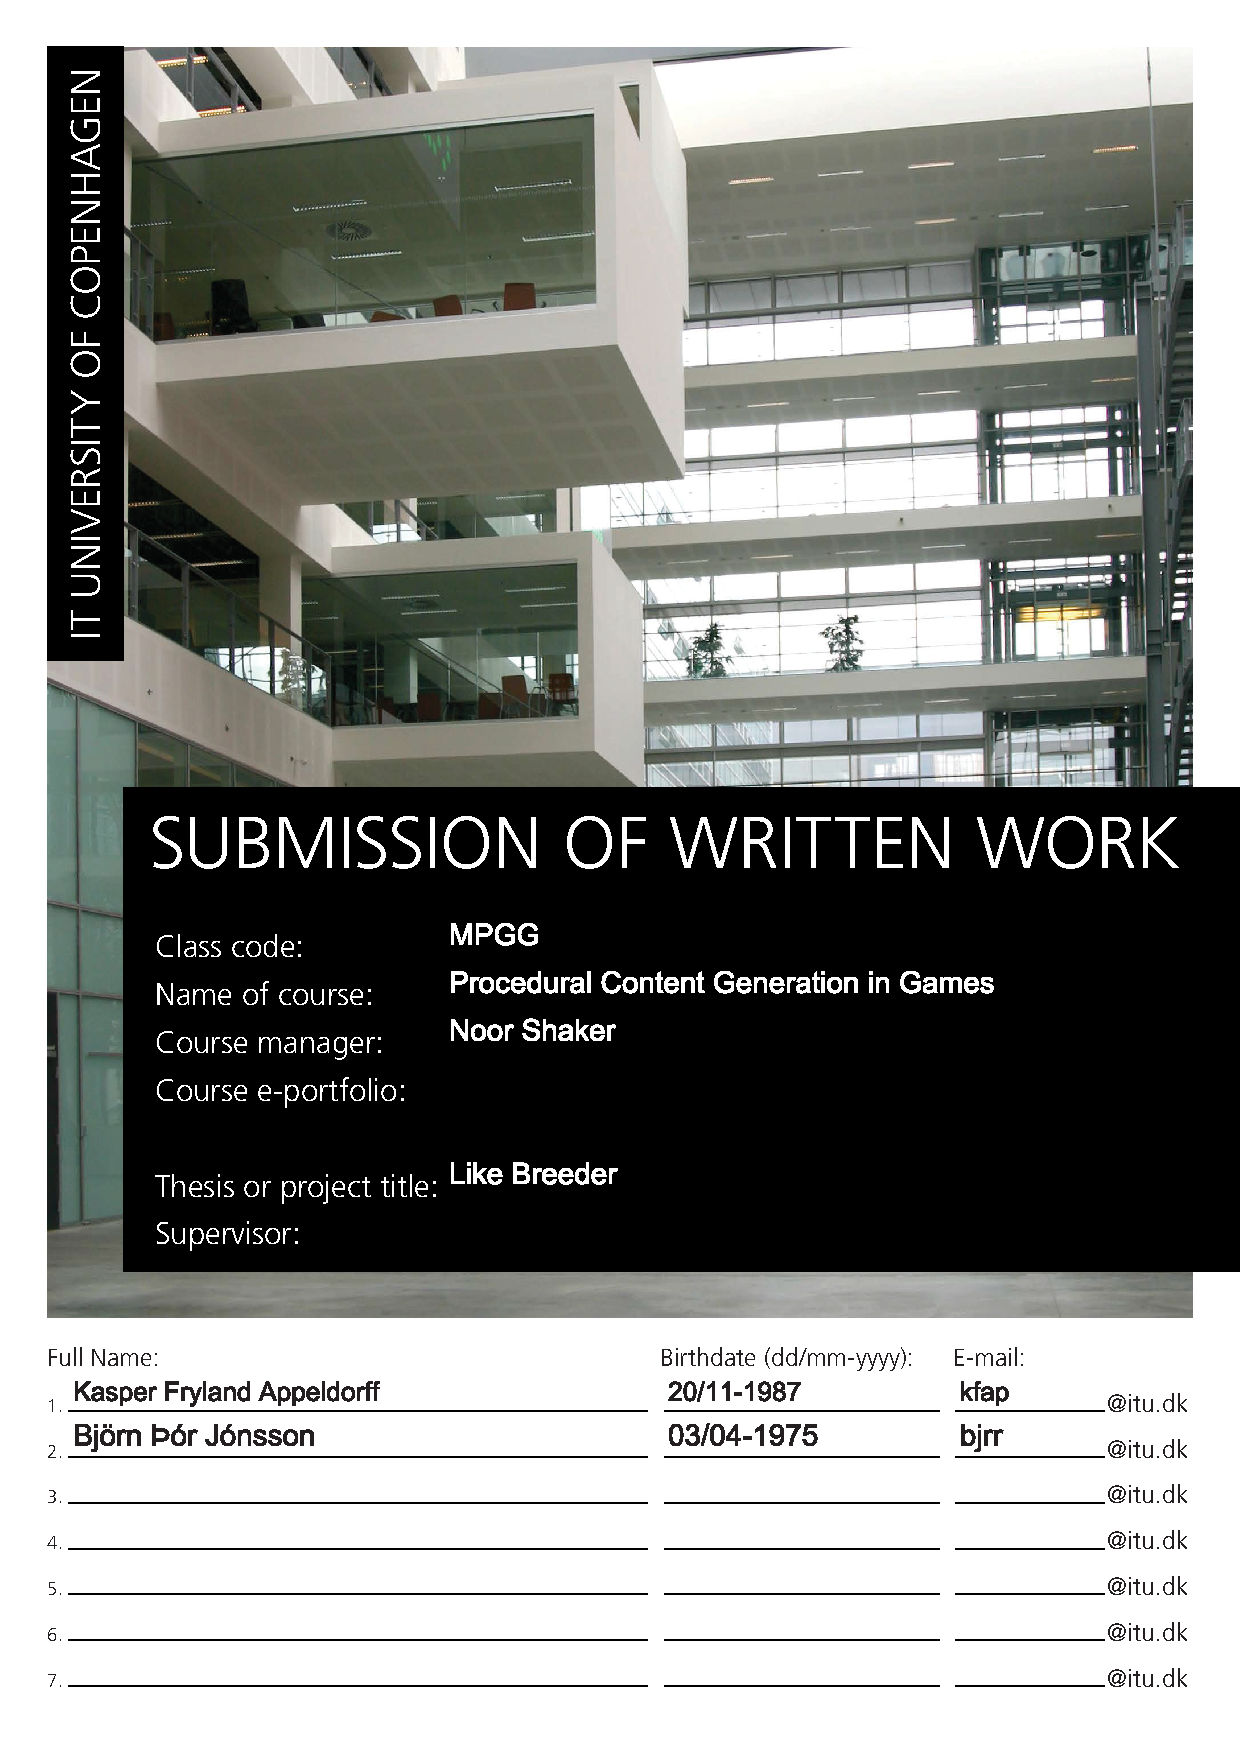
\includepdf{frontpage.pdf}
%\tableofcontents %Table of contents. Automagic
%\listoffigures %Also has \listoftables
\listoftodos % Requires package todonotes
\newpage
\begin{abstract}
This is nice when you write something and you are not done \todo{I should totally put something here}
\begin{figure}[h!]
\missingfigure{Some sort of descripton of what should be there} %Nice if you haven't made the picture yet
\caption{hey}
\label{fig:test}
\end{figure}
\end{abstract}

\section{Introduction}
\label{sec:Introduction}
I am referencing myself in \autoref{sec:Introduction} on page \pageref{sec:Introduction}
\section{Background}
\label{sec:Background}
\section{Game Design}
\label{sec:GameDesign}
\section{Methods}
\label{sec:Methods}
\section{Results}
\label{sec:Results}
\section{Discussion}
\label{sec:Discussion}

\bibliographystyle{unsrt}
\bibliography{references}
\end{document}
